\section{Vorlesung}
\subsection{Quantencomputer}
\definition{Quantencomputer}{
        Quantencomputer funktionieren nach quantenmechanischen Gesetzen und haben das Potential, bestimmte (aber nicht alle) Rechenaufgaben effizienter als klassische Computer zu lösen.\\
        Die heutigen (10.2025) Quantencomputer sind jedoch noch zu klein und zu fehlerbehaftet, um den klassischen überlegen zu sein. Dieser Punkt könnte jedoch irgendwann in den nächsten Jahren erreicht werden.
}
\subsection{Aufbau der Vorlesung}
Diese Vorlesung vermittelt einen Einblick in die zugrunde liegenden quantenmechanischen Gesetze, die allgemeine Funktionsweise eines Quantencomputers, und stellt für mögliche Anwendungen geeignete \b{Quantenalgorithmen} vor:
\begin{itemize}
    \item \b{Shor-Algorithmus} zur Faktorisierung großer Zahlen
    \item \b{Grover-Algorithmus} zum Auffinden eines gesuchten Elements in einer unstrukturierten Menge
    \item \b{HHL-Algorithmus} zur Lösung linearer Gleichungssysteme
    \item \b{\ac{vqe}} zur Bestimmung der Grundzustandsenergien von Molekülen (wichtig zur Berechnung chemischer Reaktionszeiten)
    \item \b{\ac{qaoa}} zur Lösung von Optimierungs- problemen (z.B. in der Finanzmathematik oder Logistik)
\end{itemize}
\section{Besonderheiten von Quantencomputern}
\textbf{Klassische Computer} funktionieren mit Bits (0 oder 1). Der Zustand eines klassischen Computers (genauer gesagt: seines Arbeitsspeichers) kann zu jedem Zeitpunkt durch eine Reihe von Nullen oder Einsen beschrieben werden, z.B.:
\cf{0\ 0\ 1\ 0\ 1\ 0\ 1\ 1\ 1\ 0\ 0\ 1\ 1\ 1\ 0\ 0\ 0\ 0\ 1\ \dots} 
\textbf{Quantencomputer} funktionieren mit \b{Qubits}. Ein solches Qubit hat auch zwei mögliche Zustände, die mit \ket{0} und \ket{1} bezeichnet werden. Dies können z.B. verschiedene elektronische Zustände eines Atoms sein:

\begin{figure}[h!]
    \centering
    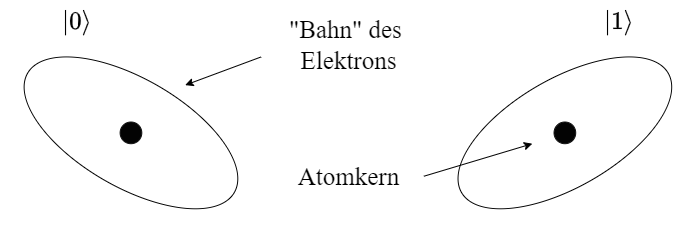
\includegraphics[width=.4\textwidth]{images/bahnen.png}
    \caption{In der QM gibt es eigentlich keine "Bahnen"! Gezeigt werden soll: Im Zustand \ket{0} bzw. \ket{1} hält sich das Elektron mit unterschiedlichen Wahrscheinlichkeiten an verschiedenen Orten auf.}
\end{figure}

Nach den Gesetzen der \ac{qm} sind jedoch auch Überlagerungen ("Superpositionen") dieser beiden Zustände möglich:
\cf{
    \cket{\psi} = a_0\cket{0}+a_1\cket{1}\quad\textrm{, wobei } a_0,a_1\in\mathbb{C} 
}
Das Qubit befindet sich dann gewissermaßen "gleichzeitig" in Zustand \ket{0} und \ket{1}. Versucht man, durch Messung, den Zustand auszulesen, so ist es allgemein unmöglich, das Ergebnis der Messung mit Sicherheit vorherzusagen: Man findet entweder das Ergebnis "\ket{0}" (mit Wahrscheinlichkeit \f{|a_0|^2}), oder "\ket{1}" (mit Wahrscheinlichkeit \f{|a_1|^2}). Daher muss gelten: \f{|a_0|^2+|a_1|^2=1}\\

Zustände mehrerer Qubits haben entsprechend folgende Form:
\begin{align*}
    \text{2 Qubits: }\cket{\psi} =\ & a_{00}\cket{00}+a_{01}\cket{01}+a_{10}\cket{10}+a_{11}\cket{11}\quad&\Rightarrow\ &4=2^2\text{ komplexe Zahlen nötig,}\\
    &&& \text{ um Zustand zu beschreiben}\\
    \text{3 Qubits: }\cket{\psi} =\ & a_{000}\cket{000}+a_{001}\cket{001}+a_{010}\cket{010}+a_{011}\cket{011}+&\\
    &a_{100}\cket{100}+a_{101}\cket{101}+a_{110}\cket{110}+a_{111}\cket{111}\quad&\Rightarrow\ &2^3 = 8\\
    \text{n Qubits: }\cket{\psi} =\ & a_{00\dots00}\cket{00\dots00}+a_{00\dots01}\cket{00\dots01}+\dots &\Rightarrow\ & 2^n
\end{align*}
Für großes \f{n} ist es daher unmöglich, einen Quantencomputer auf einem klassischen Computer zu simulieren, da der Speicher nicht ausreicht, um alle Koeffizienten \f{a_{00\dots00}, a_{00\dots01}, \dots} zu speichern. In der Praxis ist dieser Punkt zur Zeit bei \f{n\approx 60} erreicht, theoretisch spätestens bei \f{n=160}, da \f{2^{160} \approx 10^{48}} ungefähr \f{\frac{1}{10}} der Anzahl der Atome in der Erde entspricht.\\

\b{Aber:} Eine Überlagerung von \f{2^n} Zuständen an sich ist nicht hilfreich, da beim Auslesen zum Schluss nur einer dieser Zustände als Ergebnis auftritt (z.B. Ergebnis "\f{00\dots00}" mit Wahrscheinlichkeit \f{|a_{00\dots00}|^2}). Quantenalgorithmen müssen also so konstruiert werden, dass nur die gewünschten Ergebnisse (d.h. die Lösungen des gegebenen Problems) mit hoher Wahrscheinlichkeit auftreten. Dies ist schwierig, und bislang gibt es nur für einige spezielle Probleme geeignete Algorithmen.\\

\b{Außerdem:} Quantenmechanische Überlagerungen sind sehr empfindlich gegenüber Störungen. Die Qubits müssen extrem gut von ihrer Umgebung isoliert werden, was in der Praxis schwierig zu be- werkstelligen ist.

\section{Quantenmechanische Grundlagen}
\subsection{Lineare Algebra}
\definition{Vektorraum}{
    Vektoren eines \f{N}-dimensionalen komplexen Vektorraums \f{V} mit Basis \f{B = (v_1, v_2, \dots, v_n)} haben folgende Form:
    \cf{
        v = a_1v_1+a_2v_2+\dots+a_Nv_N = \begin{pmatrix}
            a_1\\a_2\\\vdots\\a_N
        \end{pmatrix} \quad\leftarrow\quad \begin{matrix}
            \text{(Darstellung des Vektors }v\\\text{bzgl. Basis }v_1, v_2, \dots, v_N)
        \end{matrix}
    }
    \b{Addition \& Skalarmultiplikation: }
    \cf{
        \begin{pmatrix}
            a_1\\a_2\\\vdots\\a_N
        \end{pmatrix} + \begin{pmatrix}
            b_1\\b_2\\\vdots\\b_N
        \end{pmatrix} = \begin{pmatrix}
            a_1+b_1\\a_2+b_2\\\vdots\\a_N+b_N
        \end{pmatrix} \quad;\quad
        \lambda\begin{pmatrix}
            a_1\\a_2\\\vdots\\a_N
        \end{pmatrix} = \begin{pmatrix}
            \lambda a_1\\\lambda a_2\\\vdots\\\lambda a_N
        \end{pmatrix} \quad;\quad a_1, \dots, a_N \in \mathbb{C}
    }
}
\definition{Komplexe Konjugation}{
    Eine komplexe Zahl \f{z} kann wie folgt komplex konjugiert werden:
    \f{
        z = a + bi \mapsto z^* = \bar{z} = a - bi
    }
}
\definition{Lineare Operatoren (Matrizen)}{
    Ein linearer Operator \f{A} hat folgende Eigenschaften:
    \begin{gather*}
        A:V \mapsto Av\in V\\
        A(v+w) = Av+Aw\\
        A(\lambda v) = \lambda (Av)
    \end{gather*}
    \b{Matrizenmultiplikation:}
    \cf{
        (AB)v = A(Bv) \quad\implies\quad \text{bekannte Regel für Multiplikation zweier Matrizen}
    }
    \b{Adjungierter Operator:}
    \cf{
        \quad A^\dagger = (A^*)^\top = \begin{pmatrix}
            A_{11}^* & \dots & A_{N1}^* \\
            \vdots & \ddots & \vdots \\
            A_{1N}^* & \dots & A_{NN}^* 
        \end{pmatrix} \quad,\quad
        (AB)^\dagger = B^\dagger A^\dagger \quad,\quad
        (\lambda A)^\dagger = \lambda^*A^\dagger
    }
}
\definition{Besondere Operatoren}{
    \begin{itemize}
        \item Selbstadjungierter Operator: \f{A=A^\dagger}
        \item Unitärer Operator \f{U}: \f{UU^\dagger = U^\dagger U = \mathbb{I}}
        \item Projektor \f{P}: \f{P=P^\dagger} und \f{P^2=p}
    \end{itemize}
}
\definition{Skalarprodukt}{
    \cf{
        v = \begin{pmatrix}
            a_1 \\ \vdots \\ a_N
        \end{pmatrix}, w = \begin{pmatrix}
            b_1 \\ \vdots \\ b_N
        \end{pmatrix} \implies \left\langle v,w \right\rangle = v^\dagger w = (a_1^*,\dots,a_N^*)\begin{pmatrix}
            b_1\\ \vdots \\ b_N
        \end{pmatrix} = a_1^*b_1+\dots+a_N^*b_N
    }
    Es gelten folgende Rechenregeln:
    \begin{gather*}
        \left\langle u,v+w\right\rangle = \left\langle u,v\right\rangle + \left\langle u,w\right\rangle   \\
        \left\langle u, \lambda v\right\rangle = \lambda \left\langle u,v\right\rangle  \\
        \left\langle u,v\right\rangle = \left\langle v,u\right\rangle^*  \\
        \implies \left\langle u+v,w\right\rangle = \left\langle u,w\right\rangle + \left\langle v,w\right\rangle \quad,\quad \left\langle \lambda u,v\right\rangle = \lambda^*\left\langle u,v\right\rangle \quad,\quad \left\langle u,Av\right\rangle = \left\langle A^\dagger u,v\right\rangle   
    \end{gather*}
}
\definition{Weitere Begriffe}{
    \begin{itemize}
        \item \b{Norm:} \f{\left\lVert v\right\rVert \sqrt{\left\langle v,v\right\rangle } \geq 0 \quad (\left\lVert v\right\rVert = 0 \Leftrightarrow v = 0 )}
        \item \b{Orthonormalbasis:} \f{
            (v_1,\dots,v_N): \left\langle v_i,v_j\right\rangle = \delta_{ij} = \begin{cases}1 \text{ falls } i=j\\0 \text{ falls } i\neq j\end{cases} 
            }
        \item Für unitäre Matrizen U gilt: \f{\left\lVert Uv\right\rVert = \left\lVert v\right\rVert  }
    \end{itemize}    
}
\definition{Eigenwerte und Eigenvektoren}{
    \begin{itemize}
        \item \f{v} ist \ac{ev} von \f{A} mit \ac{ew} \f{\lambda \Leftrightarrow Av = \lambda v}
        \item Eine selbstadjungierte Matrix ist \b{unitär diagonalisierbar}, d.h. es gibt eine unitäre Matrix \f{U}, sodass \f{U^\dagger AU = \begin{pmatrix}
            \lambda_1 & & 0\\
            & \ddots & \\
            0 & & \lambda_N
        \end{pmatrix}}. \f{w_i = Uv_i} ist dann \ac{ev} von \f{A} mit \ac{ew} \f{\lambda_i \in \mathbb{R}}.
        \item Auch unitäre Matrizen sind unitär diagonalisierbar. Ihre \ac{ew} sind komplexe Zahlen mit Betrag \f{1}, d.h. \f{\lambda_k = e^{i\varphi_k}, \varphi_k\in\mathbb{R}}.
        \item Die \ac{ew} von \f{A} können durch Lösung folgender Gleichung berechnet werden: \f{\det(A-\lambda\mathbb{I}) = 0}
    \end{itemize}
}
\definition{Tensorprodukt}{
    Ist \f{\left\{v_i|i=1,\dots,N\right\} } eine Basis von \f{V} (dim\f{V=N}) und \f{\left\{w_i|i=1,\dots,M\right\} } eine Basis von \f{W} (dim\f{W=M}), so bildet \f{\left\{v_i\otimes w_j|i=1,\dots,N;j=1,\dots,M\right\}} eine Basis von \f{V\otimes W} mit dim\f{V\otimes W = NM}.    
    \b{Beispiel:}
    \cf{
        \left.\begin{array}{r}
            (v_1, v_2) \text{ Basis von }V\\
            (w_1,w_2,w_3)\text{ Basis von }W
        \end{array}\right\}\Rightarrow (v_1\otimes w_1, v_1\otimes w_2, v_1\otimes w_3, v_2\otimes w_1, v_2\otimes w_2, v_2\otimes w_3)
    }
    Für beliebige Vektoren \f{u,v\in V} und \f{w,x\in W} und \f{\lambda \in \mathbb{C}} gilt defintionsgemäß:
    \cf{
        \left.\begin{aligned}
            (\lambda v)\otimes w = v\otimes(\lambda w) = \lambda (v\otimes w) &\quad\\
            (u+v)\otimes w = u\otimes w + v\otimes w&\quad\\
            v\otimes (w+x) = v\otimes w + v\otimes x &\quad\\
    \end{aligned}\right\rvert \Rightarrow\quad
        v = \begin{pmatrix}
            a_1\\\vdots\\a_N
        \end{pmatrix},\quad
        w = \begin{pmatrix}
            b_1\\\vdots\\b_M
        \end{pmatrix}\quad v\otimes w = \begin{pmatrix}
            a_1b_1\\
            \dots\\
            a_1b_M\\
            a_2b_1\\
            \dots\\
            a_Nb_M
        \end{pmatrix}
    }
    \b{Verschränkung:}\\
    Falls ein Vektor \f{z\in V\otimes W} als ein Produkt zweier Vektoren \f{v\in V} und \f{w\in W} geschrieben werden kann (\f{z = v\otimes w}) so heißt \f{z} \b{Produktvektor}. Falls nicht, heißt \f{z} \b{verschränkt}.\\

    \b{Tensorprodukt von Operatoren:}\\
    Definiert als \f{(A\otimes B)(v\otimes w) := (Av)\otimes(Bw)}. Hieraus ergibt sich eine (naheliegende) Vorschrift zur Bestimmung der Matrixelemente von \f{A\otimes B}:
    \cf{
        A\otimes B = \begin{pmatrix}
            A_{11}B & \dots & A_{M1}B \\
            \vdots & \ddots & \vdots \\
            A_{1N}B & \dots & A_{MN}B
        \end{pmatrix}
    }
}
